\documentclass[12pt, a4paper]{report}

% Packages :

\usepackage[french]{babel}
\usepackage[utf8]{inputenc}
\usepackage[T1]{fontenc}
\usepackage[pdftex, pdfauthor={Bacomathiques}]{hyperref}
\usepackage{sectsty}
\usepackage[explicit]{titlesec}
\usepackage{xcolor}
\usepackage{amsmath}
\usepackage{amssymb}
\usepackage{amsthm}
\usepackage{fourier}
\usepackage{titlesec}
\usepackage{fancyhdr}
\usepackage{catchfilebetweentags}
\usepackage[french, capitalise, noabbrev]{cleveref}
\usepackage[fit, breakall]{truncate}
\usepackage[margin=3cm]{geometry}
\usepackage{tocloft}
\usepackage{tikz}
\usepackage{tocloft}
\usepackage{microtype}
\usepackage{listings}
\usepackage{tabularx}
\usepackage{calc}
\usepackage[export]{adjustbox}
\usepackage[most]{tcolorbox}
\usepackage{standalone}
\usepackage{xlop}
\usepackage{etoolbox}
\usepackage{environ}

\usetikzlibrary{arrows.meta}
\usetikzlibrary{trees}

% Paramètres :

\author{Bacomathiques}
\definecolor{graphe}{HTML}{93c9ff}
\setcounter{MaxMatrixCols}{12}
\setlength{\parindent}{0pt}
\setlength{\fboxsep}{0pt}
%\pdfsuppresswarningpagegroup=1

% Code :

\lstdefinestyle{style}{
	backgroundcolor=\color{white},
	commentstyle=\em\color[HTML]{999988},
	keywordstyle=\bfseries,
	identifierstyle=\normalfont,
	stringstyle=\color[rgb]{0.87, 0.07, 0.27},
	basicstyle=\ttfamily\color{black},
	breakatwhitespace=false,
	breaklines=true,
	captionpos=b,
	keepspaces=true,
	numbers=left,
	numbersep=5pt,
	showspaces=false,
	showstringspaces=false,
	showtabs=false,
	tabsize=2,
	numbers=none
}

\lstset{style=style}
\lstset{
	literate=
	{á}{{\'a}}1
	{à}{{\`a}}1
	{ã}{{\~a}}1
	{é}{{\'e}}1
	{ê}{{\^e}}1
	{í}{{\'i}}1
	{ó}{{\'o}}1
	{õ}{{\~o}}1
	{ú}{{\'u}}1
	{ü}{{\"u}}1
	{ç}{{\c{c}}}1
}

\lstset{
	framextopmargin=10pt,
	framexrightmargin=10pt,
	framexbottommargin=10pt,
	framexleftmargin=10pt,
	xleftmargin=10pt,
	xrightmargin=10pt,
}

% Couleurs :

\definecolor{title}{HTML}{912c21}
\definecolor{section}{HTML}{1c567d}
\definecolor{subsection}{HTML}{2980b9}

\definecolor{rule}{HTML}{c4c4c4}

\definecolor{formula}{HTML}{ebf3fb}
\definecolor{formula-left}{HTML}{3583d6}

\definecolor{tip}{HTML}{dcf3d8}
\definecolor{tip-left}{HTML}{26a65b}

\definecolor{demonstration}{HTML}{fff8de}
\definecolor{demonstration-left}{HTML}{f1c40f}

\definecolor{exercise}{HTML}{e0f2f1}
\definecolor{exercise-left}{HTML}{009688}

\definecolor{correction}{HTML}{e0f7fa}
\definecolor{correction-left}{HTML}{00bcd4}

\definecolor{toc}{HTML}{fceae9}
\definecolor{toc-left}{HTML}{e74c3c}
\definecolor{toc-dark}{HTML}{87281f}

% Titres :

\renewcommand{\thesection}{\Roman{section} - }
\renewcommand{\thesubsection}{\arabic{subsection}. }

\newcommand{\sectionstyle}{\normalfont\LARGE\bfseries\color{section}}
\titleformat{\section}{\sectionstyle}{\thesection #1}{0pt}{}
\titleformat{name=\section, numberless}{\sectionstyle}{#1}{0pt}{}

\newcommand{\subsectionstyle}{\normalfont\Large\bfseries\color{subsection}}
\titleformat{\subsection}{\subsectionstyle}{\thesubsection #1}{0pt}{}
\titleformat{name=\subsection, numberless}{\subsectionstyle}{#1}{0pt}{}

\titlelabel{\thetitle\ }

% Table des matières :

\addto\captionsfrench{\renewcommand\contentsname{}}
\renewcommand{\cftsecpagefont}{\color{toc-dark}}
\renewcommand{\cftsubsecpagefont}{\color{toc-dark}}
\renewcommand{\cftsecleader}{\cftdotfill{\cftdotsep}}
\renewcommand{\cftsecfont}{\bfseries}
\renewcommand{\cftsecpagefont}{\bfseries\color{toc-dark}}
\setlength{\cftbeforetoctitleskip}{0pt}
\setlength{\cftaftertoctitleskip}{0pt}
\setlength{\cftsecindent}{0pt}
\setlength{\cftsubsecindent}{20pt}
\setlength{\cftsubsecnumwidth}{20pt}

% Commandes :

\newcommand{\newpar}{\\[\medskipamount]}
\newcommand{\lesson}[3]{%
	\newcommand{\level}{#1}%
	\newcommand{\id}{#2}%
	\hypersetup{pdftitle={#3}}
	\begin{center}%
		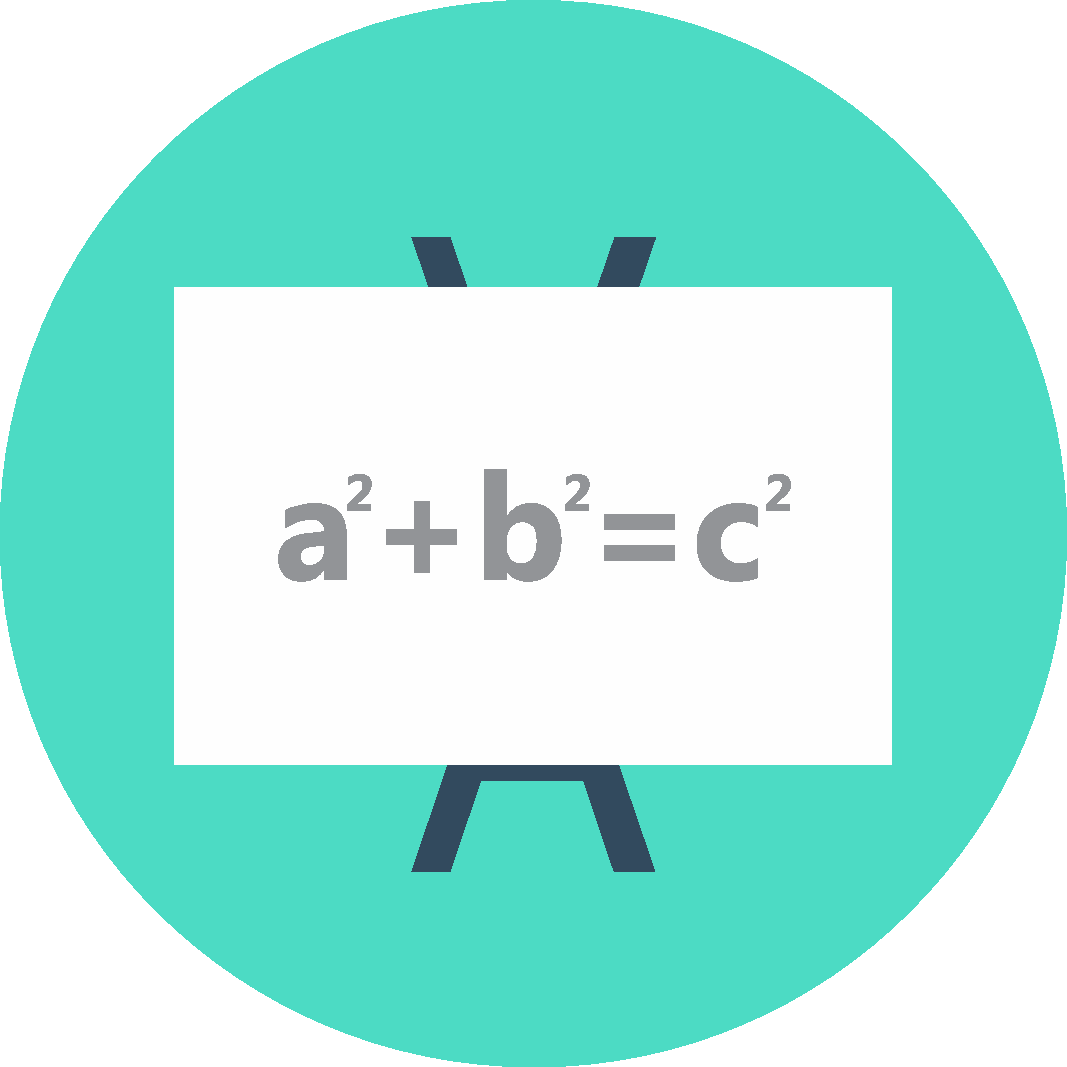
\includegraphics[width=150px]{\imagespath/bacomathiques}%
		
		\vspace{30pt}%
		{\Huge\color{title} #3}%
		
		\vspace{10pt}%
		{Bacomathiques --- \href{https://bacomathiqu.es/cours/#1/#2}{\color{section} https://bacomathiqu.es}}%
		
		\vspace{20pt}%
	\end{center}%
	\begin{toc}
		\tableofcontents%
	\end{toc}
	\thispagestyle{empty}%
	\newpage%
	\setcounter{page}{1}%
}
\newcommand{\imagespath}{../../images}
\newcommand{\lessonimagespath}{\imagespath/lessons/\level/\id/}
\newcommand{\includelatexpicture}[2][\textwidth - 100pt]{%
	\begin{center}%
		\resizebox{#1}{!}{%
			\input{\lessonimagespath#2}%
		}%
	\end{center}%
	\medskip%
}
\newcommand{\includeimage}[1]{%
	\begin{center}%
		\includegraphics{\lessonimagespath#1}%
	\end{center}%
	\medskip%
}
\newcommand{\includerepresentation}[1]{%
	\begin{center}%
		\setlength{\fboxrule}{0.5pt}%
		\href{https://www.geogebra.org/m/#1}{\includegraphics[width=\textwidth-1pt,fbox]{\lessonimagespath#1}}%
	\end{center}%
}
\newcommand{\floor}[1]{\lfloor #1 \rfloor}

\makeatletter
\newcommand\inputcontent{\@ifstar{\inputcontent@star}{\inputcontent@nostar}}
\newcommand{\inputcontent@star}[1]{%
	\ExecuteMetaData[#1]{content}%
}
\newcommand{\inputcontent@nostar}[1]{%
	\newpage%
	\inputcontent@star{#1}%
}
\makeatother

\let\oldsection\section
\renewcommand\section{\clearpage\oldsection}
\newcommand{\contentwidth}[1][medium]{}

% En-têtes :

\pagestyle{fancy}

\renewcommand{\sectionmark}[1]{\markboth{\thesection \ #1}{}}

\fancyhead[R]{\truncate{0.23\textwidth}{\color{title}\thepage}}
\fancyhead[L]{\truncate{0.73\textwidth}{\color{title}\leftmark}}
\fancyfoot[C]{\scriptsize \href{https://bacomathiqu.es/cours/\level/\id}{\texttt{bacomathiqu.es}}}

\makeatletter
\patchcmd{\f@nch@head}{\rlap}{\color{rule}\rlap}{}{}
\patchcmd{\headrule}{\hrule}{\color{rule}\hrule}{}{}
\makeatother

% Environnements :

\newenvironment{nosummary}{}{}
\newcommand{\tcolorboxtitle}[2]{\setlength{\fboxsep}{2.5pt}\hspace{-10pt}\colorbox{#1-left}{\hspace{8pt}\MakeUppercase{#2} \hspace{2pt} \includegraphics[height=0.8em]{\imagespath/bubbles/#1}\hspace{5pt}}}
\newcommand{\tcolorboxsubtitle}[2]{\ifstrempty{#2}{}{\textcolor{#1-left}{\large#2}\\[\medskipamount]}}
\tcbset{
	frame hidden,
	boxrule=0pt,
	boxsep=0pt,
	enlarge bottom by=8.5pt,
	enhanced jigsaw,
	boxed title style={sharp corners,boxrule=0pt,coltitle={white},titlerule=0pt},
	fonttitle=\fontsize{6pt}{6pt}\bfseries\boldmath,
	top=10pt,
	right=10pt,
	bottom=10pt,
	left=10pt,
	arc=0pt,
	outer arc=0pt,
}
\newtcolorbox{toc}[1][]{
	colback=toc,
	borderline west={3pt}{0pt}{toc-left},
	title=\tcolorboxtitle{toc}{Table des matières},
	colbacktitle=toc,
	before upper={\tcolorboxsubtitle{toc}{#1}}
}
\newtcolorbox{formula}[1][]{
	colback=formula,
	borderline west={3pt}{0pt}{formula-left},
	title=\tcolorboxtitle{formula}{À retenir},
	colbacktitle=formula,
	before upper={\tcolorboxsubtitle{formula}{#1}}
}
\newtcolorbox{tip}[1][]{
	colback=tip,
	borderline west={3pt}{0pt}{tip-left},
	title=\tcolorboxtitle{tip}{À lire},
	colbacktitle=tip,
	before upper={\tcolorboxsubtitle{tip}{#1}}
}
\newtcolorbox{demonstration}[1][]{
	colback=demonstration,
	borderline west={3pt}{0pt}{demonstration-left},
	title=\tcolorboxtitle{demonstration}{Démonstration},
	colbacktitle=demonstration,
	before upper={\tcolorboxsubtitle{demonstration}{#1}}
}

\NewEnviron{whitetabularx}[1]{%
	\renewcommand{\arraystretch}{2.5}
	\colorbox{white}{%
		\begin{tabularx}{\textwidth}{#1}%
			\BODY%
		\end{tabularx}%
	}%
}

% Longueurs :

\newlength{\espacetitreliste}
\setlength{\espacetitreliste}{-16pt}
\newcommand{\entretitreetliste}{\vspace{\espacetitreliste}}

\begin{document}
	%<*content>
	\lesson{premiere}{7}{probabilites}{Probabilités}

	\header{caption}{Les jeux de hasard sont un très bon exemple de l'utilisation des probabilités
		dans la vie courante.}

	\header{excerpt}{La théorie des probabilités est l'étude des phénomènes caractérisés par le
		hasard et l'incertitude. Elle forme avec la statistique les deux sciences du hasard
		qui sont partie intégrante des mathématiques. Ici, nous allons apprendre à représenter
		des situations de probabilités à l'aide d'un arbre mais nous allons également introduire
		quelques concepts importants comme celui de variable aléatoire ou celui de loi de
		probabilité par exemple.}

	\header{difficulty}{3}

	\section{Probabilités conditionnelles}

	\subsection{Définition}

	\begin{formula}[Définition]
		Soient $A$ et $B$ deux événements avec $A$ de probabilité non nulle. Alors \textbf{la probabilité conditionnelle de $B$ sachant que $A$ est réalisé} (notée $P_{A}(B)$) est $P_{A}(B) = \frac{P(A \cap B)}{P(A)}$.
	\end{formula}

	\begin{tip}[Rappel]
		On rappelle que $P(A \cap B) = P(A) + P(B) - P(A \cup B)$.
	\end{tip}

	\begin{tip}[Différence entre conditionnelle et intersection]
		\textbf{Il faut faire attention}, à bien faire la distinction entre une probabilité conditionnelle (``\textbf{Sachant qu'on a $A$}, quelle est la probabilité d'avoir $B$ ?'') et une intersection (``Quelle est la probabilité d'avoir \textbf{$A$ et $B$ à la fois} ?'').
	\end{tip}

	\begin{formula}[Indépendance]
		Deux événements $A$ et $B$ sont dits \textbf{indépendants} si la réalisation de l'un n'a aucune incidence sur la réalisation de l'autre et réciproquement. C'est-à-dire si $P(A \cap B) = P(A) \times P(B)$.
	\end{formula}

	\begin{formula}[Propriétés]
		Pour deux événements indépendants $A$ et $B$, on a les relations suivantes :
		\begin{itemize}
			\item $P_{A}(B) = P(B)$
			\item $P_{B}(A) = P(A)$
		\end{itemize}
	\end{formula}

	\subsection{Arbre de probabilité}

	Au lycée, pour représenter visuellement des probabilités on utilise très souvent un \textbf{arbre de probabilité}. Nous nous limiterons ici au cas de deux événements, mais il est possible d'en rajouter encore d'autres.

	Ainsi :

	\begin{formula}[Définition]
		Soient $A$ et $B$ deux événements. L'arbre de probabilité décrivant la situation est le suivant :
		\includelatexpicture{arbre-1}
	\end{formula}

	La somme (dans le sens vertical) des probabilités de chacune des branches ayant une ``racine'' commune doit toujours faire $1$.

	\begin{tip}[Exemple]
		Soit $A$ et $B$ deux événements non-indépendants tels que $P(A) = \frac{4}{7}$, $P_{A}(B) = \frac{1}{4}$ et $P_{\bar{A}}(B) = \frac{5}{9}$.
		\newline
		Alors l'arbre permettant de modéliser la situation est le suivant :
		\includelatexpicture{arbre-2}
	\end{tip}

	\subsection{Formule des probabilités totales}

	Voici maintenant l'énoncé de la \textbf{formule des probabilités totales}, qui peut être très utile pour calculer des probabilités que l'on ne connaît pas (ou qui ne sont pas données dans un énoncé d'exercice) :

	\begin{formula}[Formule des probabilités totales]
		Soient $A_1, A_2, ..., A_n$ des événements qui partitionnent (qui recouvrent) l'univers $\Omega$, alors pour tout événement $B$ :
		\[ P(B) = P(B \cap A_1) + P(B \cap A_2) + \dots + P(B \cap A_n) \]
	\end{formula}

	\begin{tip}[Exemple]
		En reprenant l'arbre précédent, comme $A$ et $\bar{A}$ recouvrent notre univers (en effet, soit on tombe sur $A$, soit on tombe sur $\bar{A}$ : pas d'autre issue possible), calculons $P(B)$ :
		\newpar
		\includelatexpicture{arbre-2}
		D'après la formule des probabilités totales, $P(B) = P(B \cap A) + P(B \cap \bar{A}) = \frac{107}{252}$.
	\end{tip}

	\section{Variables aléatoires}

	\subsection{Définition}

	\begin{formula}[Définition]
		Une \textbf{variable aléatoire} $X$ est une fonction qui, à chaque événement élémentaire de l'univers $\Omega$ y associe un nombre réel. C'est-à-dire : $X : \Omega \rightarrow \mathbb{R}$.
	\end{formula}

	L'ensemble des valeurs prises par $X$ est noté $X(\Omega)$.

	\begin{tip}
		Les variables aléatoires sont très utiles notamment pour modéliser des situations de gains ou de pertes (à un jeu d'argent par exemple).
	\end{tip}

	\subsection{Loi de probabilité}

	\begin{formula}[Définition]
		Soit $X$ une variable aléatoire. La \textbf{loi de probabilité} de $X$ attribue à chaque valeur $x_i$ la probabilité $p_i = P(X = x_i)$ de l'événement $X = x_i$ constitué de tous les événements élémentaires dont l'image par $X$ est $x_i$.
	\end{formula}

	On représente généralement les lois de probabilité par un tableau.

	\begin{formula}[Représentation d'une loi de probabilité par un tableau]
		Soit $X$ une variable aléatoire. On peut représenter sa loi de probabilité par le tableau ci-contre :
		\newpar
		\begin{whitetabularx}{|X|X|X|X|X|}
			\hline
			$x_i$ & $x_1$ & $x_2$ & ... & $x_n$ \\
			\hline
			$p_i$ \newline $= P(X = x_i)$ & $p_1$ \newline $= P(X = x_1)$ & $p_2$ \newline $= P(X = x_2)$ & ... & $p_n$ \newline $= P(X = x_n)$ \\
			\hline
		\end{whitetabularx}
		\newpar
		On a $p_1 + p_2 + \dots + p_n = 1$.
	\end{formula}

	\begin{tip}
		Cette définition peut sembler un peu compliquée mais elle signifie juste qu'une loi de probabilité assigne une probabilité à chaque valeur prise par notre variable aléatoire.
	\end{tip}

	\subsection{Espérance, variance et écart-type}

	\begin{formula}[Espérance]
		L'\textbf{espérance} $E(X)$ d'une variable aléatoire $X$ est le réel :
		\[ E(X) = x_1 \times p_1 + x_2 \times p_2 + \dots + x_n \times p_n \]
	\end{formula}

	\begin{formula}[Variance et écart-type]
		La \textbf{variance} $V(X)$ et l'\textbf{écart-type} $\sigma(X)$ d'une variable aléatoire $X$ sont les réels positifs suivants :
		\begin{itemize}
			\item $V(X) = E(X^2) - E(X)^2$
			\item $\sigma(X) = \sqrt{V(X)}$
		\end{itemize}
	\end{formula}

	\begin{tip}[Exemple]
		Calcul de l'espérance, de la variance et de l'écart-type. Soit $X$ une variable aléatoire suivant la loi de probabilité donnée par le tableau ci-dessous :
		\newpar
		\begin{whitetabularx}{|X|X|X|X|X|}
			\hline
			$x_i$ & $-1$ & $0$ & $2$ & $6$ \\
			\hline
			$p_i$ & $\frac{1}{4}$ & $\frac{1}{2}$ & $\frac{1}{8}$ & $\frac{1}{8}$ \\
			\hline
		\end{whitetabularx}
		\newpar
		On a :
		\begin{itemize}
			\item $E(X) = -1 \times \frac{1}{4} + 0 \times \frac{1}{2} + 2 \times \frac{1}{8} + 6 \times \frac{1}{8} = \frac{3}{4}$
			\item $V(X) = ((-1)^2 \times \frac{1}{4} + 0^2 \times \frac{1}{2} + 2^2 \times \frac{1}{8} + 6^2 \times \frac{1}{8}) - (\frac{3}{4})^2 = \frac{75}{16}$
			\item $\sigma(X) = \sqrt{\frac{75}{16}} \approx 2.165$
		\end{itemize}
	\end{tip}

	Chacun de ces paramètres a une utilité bien précise. En effet :

	\begin{formula}[Signification des paramètres]
		\entretitreetliste
		\begin{itemize}
			\item L'espérance est la \textbf{valeur moyenne} prise par $X$.
			\item La variance et l'écart-type mesurent la \textbf{dispersion} des valeurs prises par $X$. Plus ces valeurs sont grandes, plus les valeurs sont dispersées autour de l'espérance.
		\end{itemize}
	\end{formula}
	%</content>
\end{document}
